\documentclass[a4paper,12pt, oneside]{article}
\usepackage[utf8]{inputenc}
\usepackage[english]{babel}
\usepackage{fancyhdr}
\usepackage{geometry}
\usepackage{graphicx}
\usepackage{float} 
\usepackage{epstopdf}
\usepackage{amsmath}
\usepackage{amssymb}
\usepackage{siunitx}
\usepackage{enumitem}
\usepackage{booktabs}
\usepackage{gensymb}
\usepackage{makecell}
\usepackage{indentfirst}
\usepackage{bigints}
\usepackage{esint}
\usepackage{harpoon}
\usepackage{relsize}
\usepackage{cite}
% \usepackage{natbib}

\usepackage{subfig}
\usepackage{overpic}

\geometry{a4paper,scale = 0.8}
\pagestyle{fancy}
\fancyhead[R]{B09501028~Gauss~\textsc{Chang}}
\fancyhead[L]{\textsc{Identification of Higgs boson}}
\fancyfoot[C]{\thepage}

\setlength{\parindent}{2em}

\renewcommand{\headrulewidth}{2pt}
\renewcommand{\footrulewidth}{1pt}
% \renewcommand\thesection{\arabic {section}}
\renewcommand\thesection{\Roman{section}}
\renewcommand{\thesubsection}{\thesection.\Roman{subsection}}
\newcommand{\HRule}{\rule{\linewidth}{2pt}}

%[Lenny]
% \ChNameUpperCase
% \ChNumVar{\fontsize{80}{42}\usefont{OT1}{ptm}{m}{n}\selectfont}
% \ChTitleVar{\Huge\sc}
% \ChRuleWidth{2pt}

%Make Chapter header and footer
\makeatletter
\let\ps@plain\ps@fancy
\makeatother


%Package and definition for code demo
\usepackage{listings}
\usepackage{color}
\definecolor{dkgreen}{rgb}{0,0.6,0}
\definecolor{gray}{rgb}{0.5,0.5,0.5}
\definecolor{mauve}{rgb}{0.58,0,0.82}
\lstset{frame=single,
language=Python,
aboveskip=3mm,
belowskip=3mm,
showstringspaces=false,
columns=flexible,
basicstyle={\small\ttfamily},
numbers=left,
numberstyle=\tiny\color{gray},
keywordstyle=\color{blue},
commentstyle=\color{dkgreen},
stringstyle=\color{mauve},
breaklines=true,
breakatwhitespace=true,
tabsize=4}

% \begin{enumerate} [label = (\alph*)]
% \begin{enumerate} [label = (\roman*)]
\linespread{1.5}
\begin{document}

%---------------------------Titlepage---------------------------

\begin{titlepage}

\begin{center}


% Upper part of the page

\includegraphics[width = 0.30\textwidth]{IES_logo.pdf} \\ [1cm]
\textsc{\LARGE Institute of Earth Sciences \\ Academia Sinica} \\ [1.5cm]
\textsc{\Large Summer Internship Program} \\ [0.5cm]


% Title
\HRule \\ % [0.5cm]
{\huge \bfseries Deep Learning Based \\ Seismic Wave Identification} \\ [0.5cm]
\HRule \\ [2.5cm]

% Author and supervisor
\begin{minipage}[t]{0.4\textwidth}
\begin{flushleft} \large
\emph{Author :}\\
Gauss~\textsc{Chang} \\
% Department of Physics, NTU
\end{flushleft}
\end{minipage}
%
\begin{minipage}[t]{0.4\textwidth}
\begin{flushright} \large
\emph{Lecturer :} \\
Dr.~Kuo-Fong \textsc{Ma} \\
Dr.~Wen-Tzong \textsc{Liang} \\
\end{flushright}
\end{minipage}

\vfill

% Bottom of the page
{\large \today}

\end{center}

\end{titlepage}
\setcounter{page}{1}

% \begin{enumerate} [label = (\alph*)]
% \begin{enumerate} [label = (\roman*)]

%---------------------------Body---------------------------
\section{Abstract}
The subject is to classify particle data, e.g. a collection of high momentum Higgs boson \cite{PhysRevLett.13.508} events versus high momentum light quarks, as measured in the detector, using neural networks \cite{Giannini:2730094}.

\section{Introduction}
\begin{enumerate} [label = \Roman*.]
	\item When a ``high-momentum'' quark is produced, it will hadronize and produce a lot of particles afterwards. These particles would form an object which is called a ``Jet'', which is the product we can see in the experiments.
	\item A typical description of the jet is a collection of particles distributed in a cone. The particles are mostly hadrons, such as kaons, pions, can be either charged or neutral.
	\item When a high-momentum Higgs boson decaying into two bottom quarks, both quarks will hadronize into jets, too.
	\item However, since the initial momentum of the Higgs boson is highly ``boosted'', the open angle of the two jets is small, and would merge into single jet in the end, causing difficulties in identifying processes.
	\item That is, the Higgs jet should preserve many physics properties of the original particle, for example, the invariant mass!
\end{enumerate}
%
\begin{figure}[H]
\centering
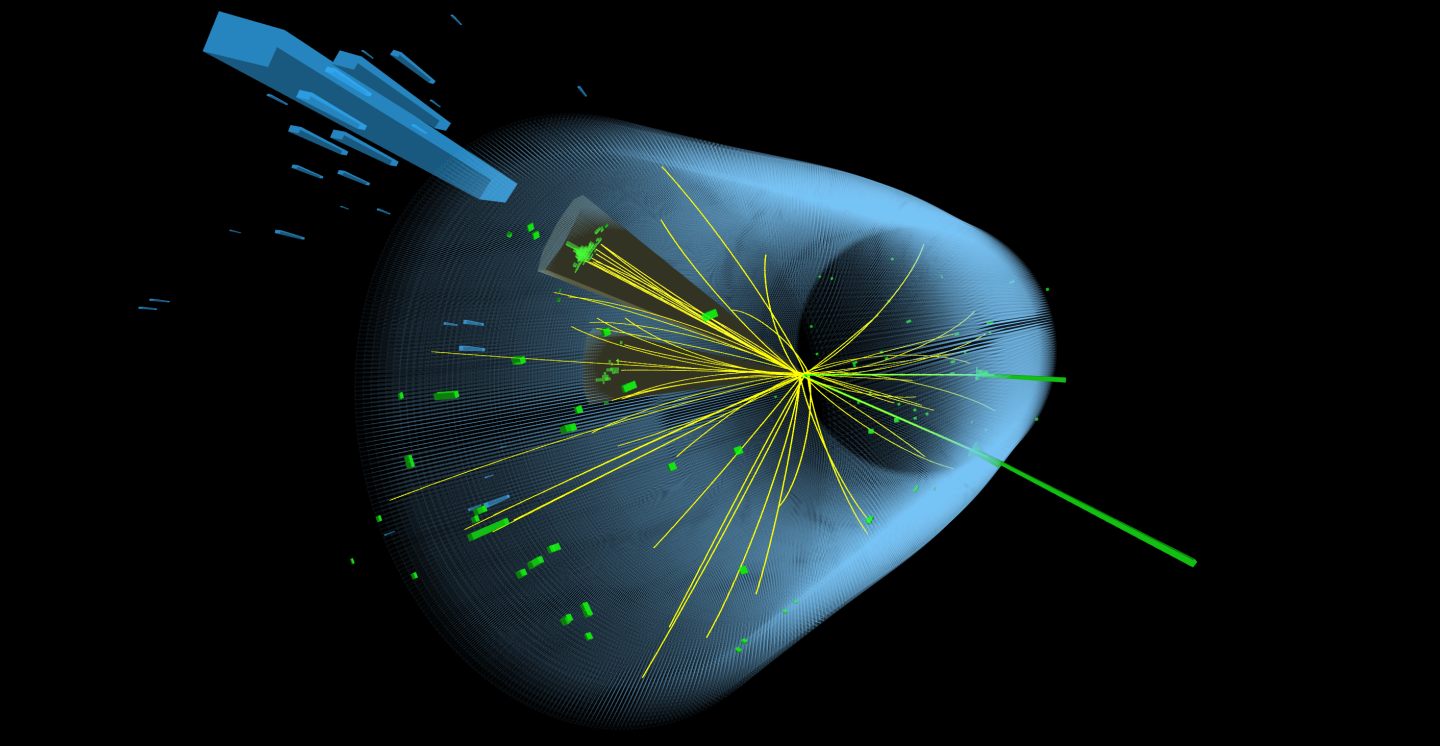
\includegraphics[width = 4in]{LHC_Sim.png}
\caption{LHC Computer Simulation}\label{LHC_Computer_Simulation}
\end{figure}

In Figure \ref{LHC_Computer_Simulation} shows how the LHC experiment look like.
%
\newpage
\subsection{Importance of this Work}
In a paper published by CERN\cite{Giannini:2730094}, they proposed a technique to use deep learning to identify the particles produced in the proton-proton collision experiment. Finding the Higgs boson is one major work. Since the higgs predicted a undiscovered boson in the 1964 \cite{PhysRevLett.13.508}, finding and proving the existence of this boson becomes the first priority of the experimental physicists. In the high energy physics field, every experiment is surprisingly expensive. Thousands of millions of data is being collected in every collision. The data scientists work on the data for years just to discover a new boson, or ``Subatomic particle''. But since the requirement of accuracy in this field is extremely high, so every new discovery must pass through the ``$5 \sigma$'' test. that means, the chance of a false discovery must be at least $5 \sigma$ out. And since every actual new discovery is a Nobel prize, timing is everything. A well-trained prediction model can tell the researchers at a early stage weather what they are speculating is true.
\subsection{Possible Model Structure}
Following is a model structure they\cite{Giannini:2730094} have proposed.
\begin{figure}[H]
\centering
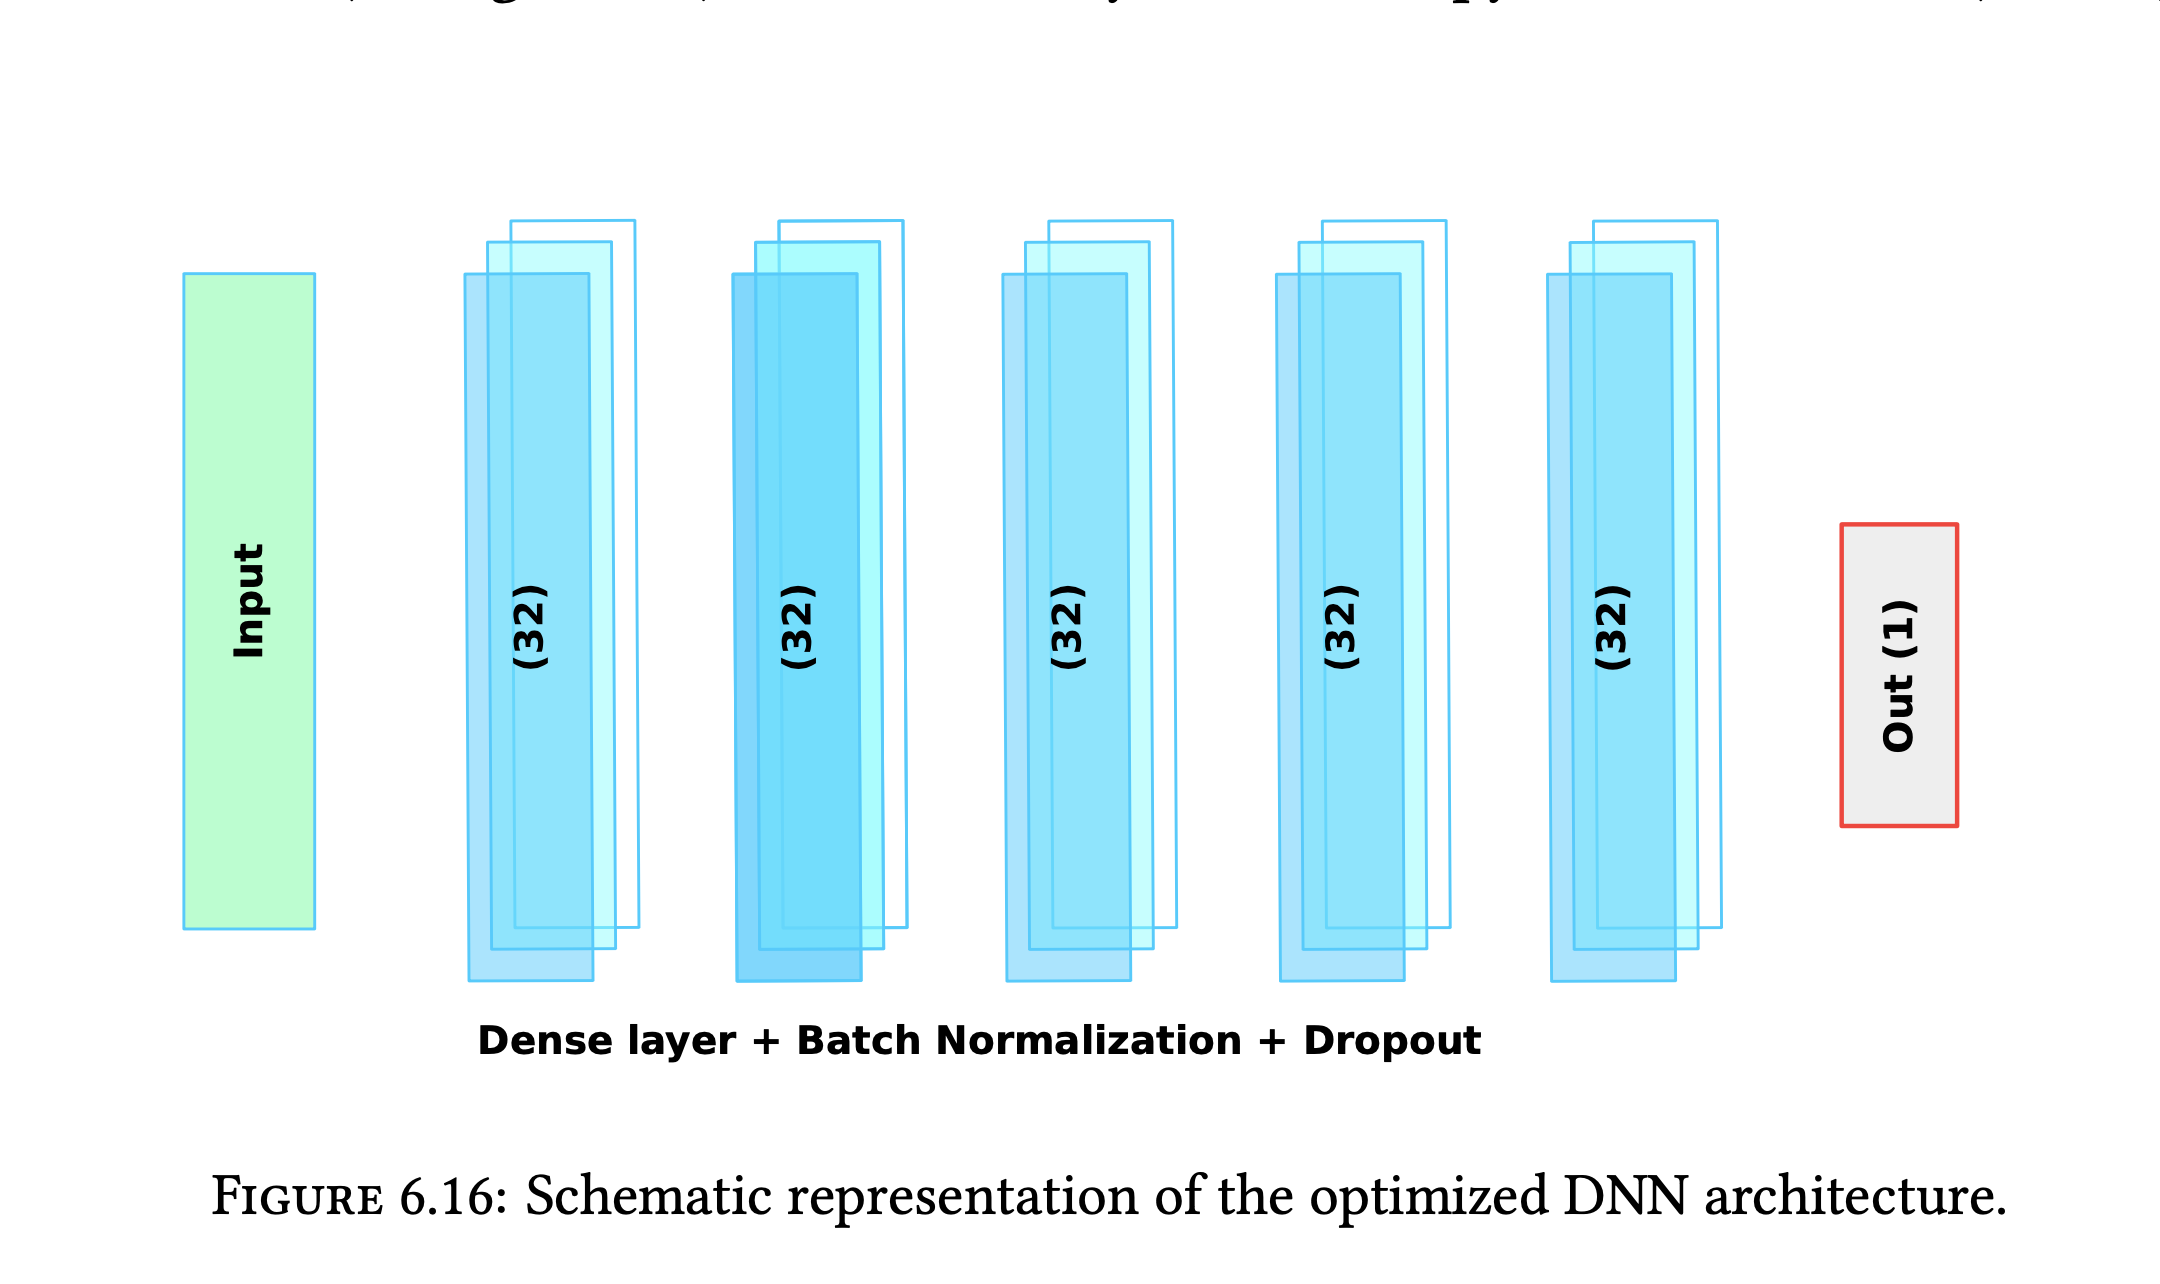
\includegraphics[width = 4in]{fig1.png}
\caption{Model Structure 1 \cite{Giannini:2730094}}\label{LHC_Computer_Simulation}
\end{figure}
\newpage
\section{Training Data Structure}

The training data structure is as shown in Table \ref{Training_Data_Structural}
%
\begin{table}[H]
\caption{Training Data Structural}\label{Training_Data_Structural}
\begin{center}
\setlength{\tabcolsep}{10pt}
\begin{tabular}{rrrrr}
\toprule
\multicolumn{1}{c}{\makecell{ID}}  & \multicolumn{1}{c}{\makecell{Code}} & \multicolumn{1}{c}{\makecell{$P_x$}} & \multicolumn{1}{c}{\makecell{$P_y$}} & \multicolumn{1}{c}{\makecell{$P_z$}} \\
\midrule
0 & 0 & -4.0379   & 1.2086  & -3.0469   \\
0 & 5 & -5.6522   & 1.6572  & -4.8261   \\
0 & 6 & -4.6699   & 1.4765  & -4.5763   \\
0 & 6 & -13.3308  & 2.4805  & -13.3598  \\
\multicolumn{5}{c}{$\vdots$} \\
\bottomrule
\end{tabular}
\end{center}
\end{table}

and the particles is represented by the code shown in Table \ref{The_Particle_Code}

\begin{table}[H]
\caption{The Particle Code}\label{The_Particle_Code}
\begin{center}
\setlength{\tabcolsep}{3pt}
\begin{tabular}{ccccccccc}
\toprule
\multicolumn{1}{c}{\makecell{Code}} & \multicolumn{1}{c}{\makecell{$0$}}  & \multicolumn{1}{c}{\makecell{$1$}} & \multicolumn{1}{c}{\makecell{$2$}} & \multicolumn{1}{c}{\makecell{$3$}} & \multicolumn{1}{c}{\makecell{$4$}} & \multicolumn{1}{c}{\makecell{$5$}} & \multicolumn{1}{c}{\makecell{$6$}} & \multicolumn{1}{c}{\makecell{$7$}} \\
\midrule
\makecell{Particle \\ name} & Photon & Electron & Position & Muon & Anti-muon & \makecell{Negatively \\ charged \\ hadron} & \makecell{Positively \\ charged \\ hadron} & \makecell{Neutral \\ hadron}  \\
Charge   & 0 & -1 & +1 & -1 & +1 & -1 & +1 & 0  \\
\bottomrule
\end{tabular}
\end{center}
\end{table}

\begin{itemize}
	\item $P_x$ is the particle momentum in $x$ direction in unit \SI{}{\GeV\per\clight}.
	\item $P_y$ is the particle momentum in $y$ direction in unit \SI{}{\GeV\per\clight}.
	\item $P_z$ is the particle momentum in $z$ direction in unit \SI{}{\GeV\per\clight}.
	\item ID stands for the event number. The same event share the same ID.
	\item This data set is obtained from Kai-Feng Chen, Detecting Boosted Higgs Competition 2022 \cite{ntuphys-cpintro-mlcomp-2022}.
\end{itemize}
\newpage
\section{Implementation}
\begin{figure}[H]
\centering
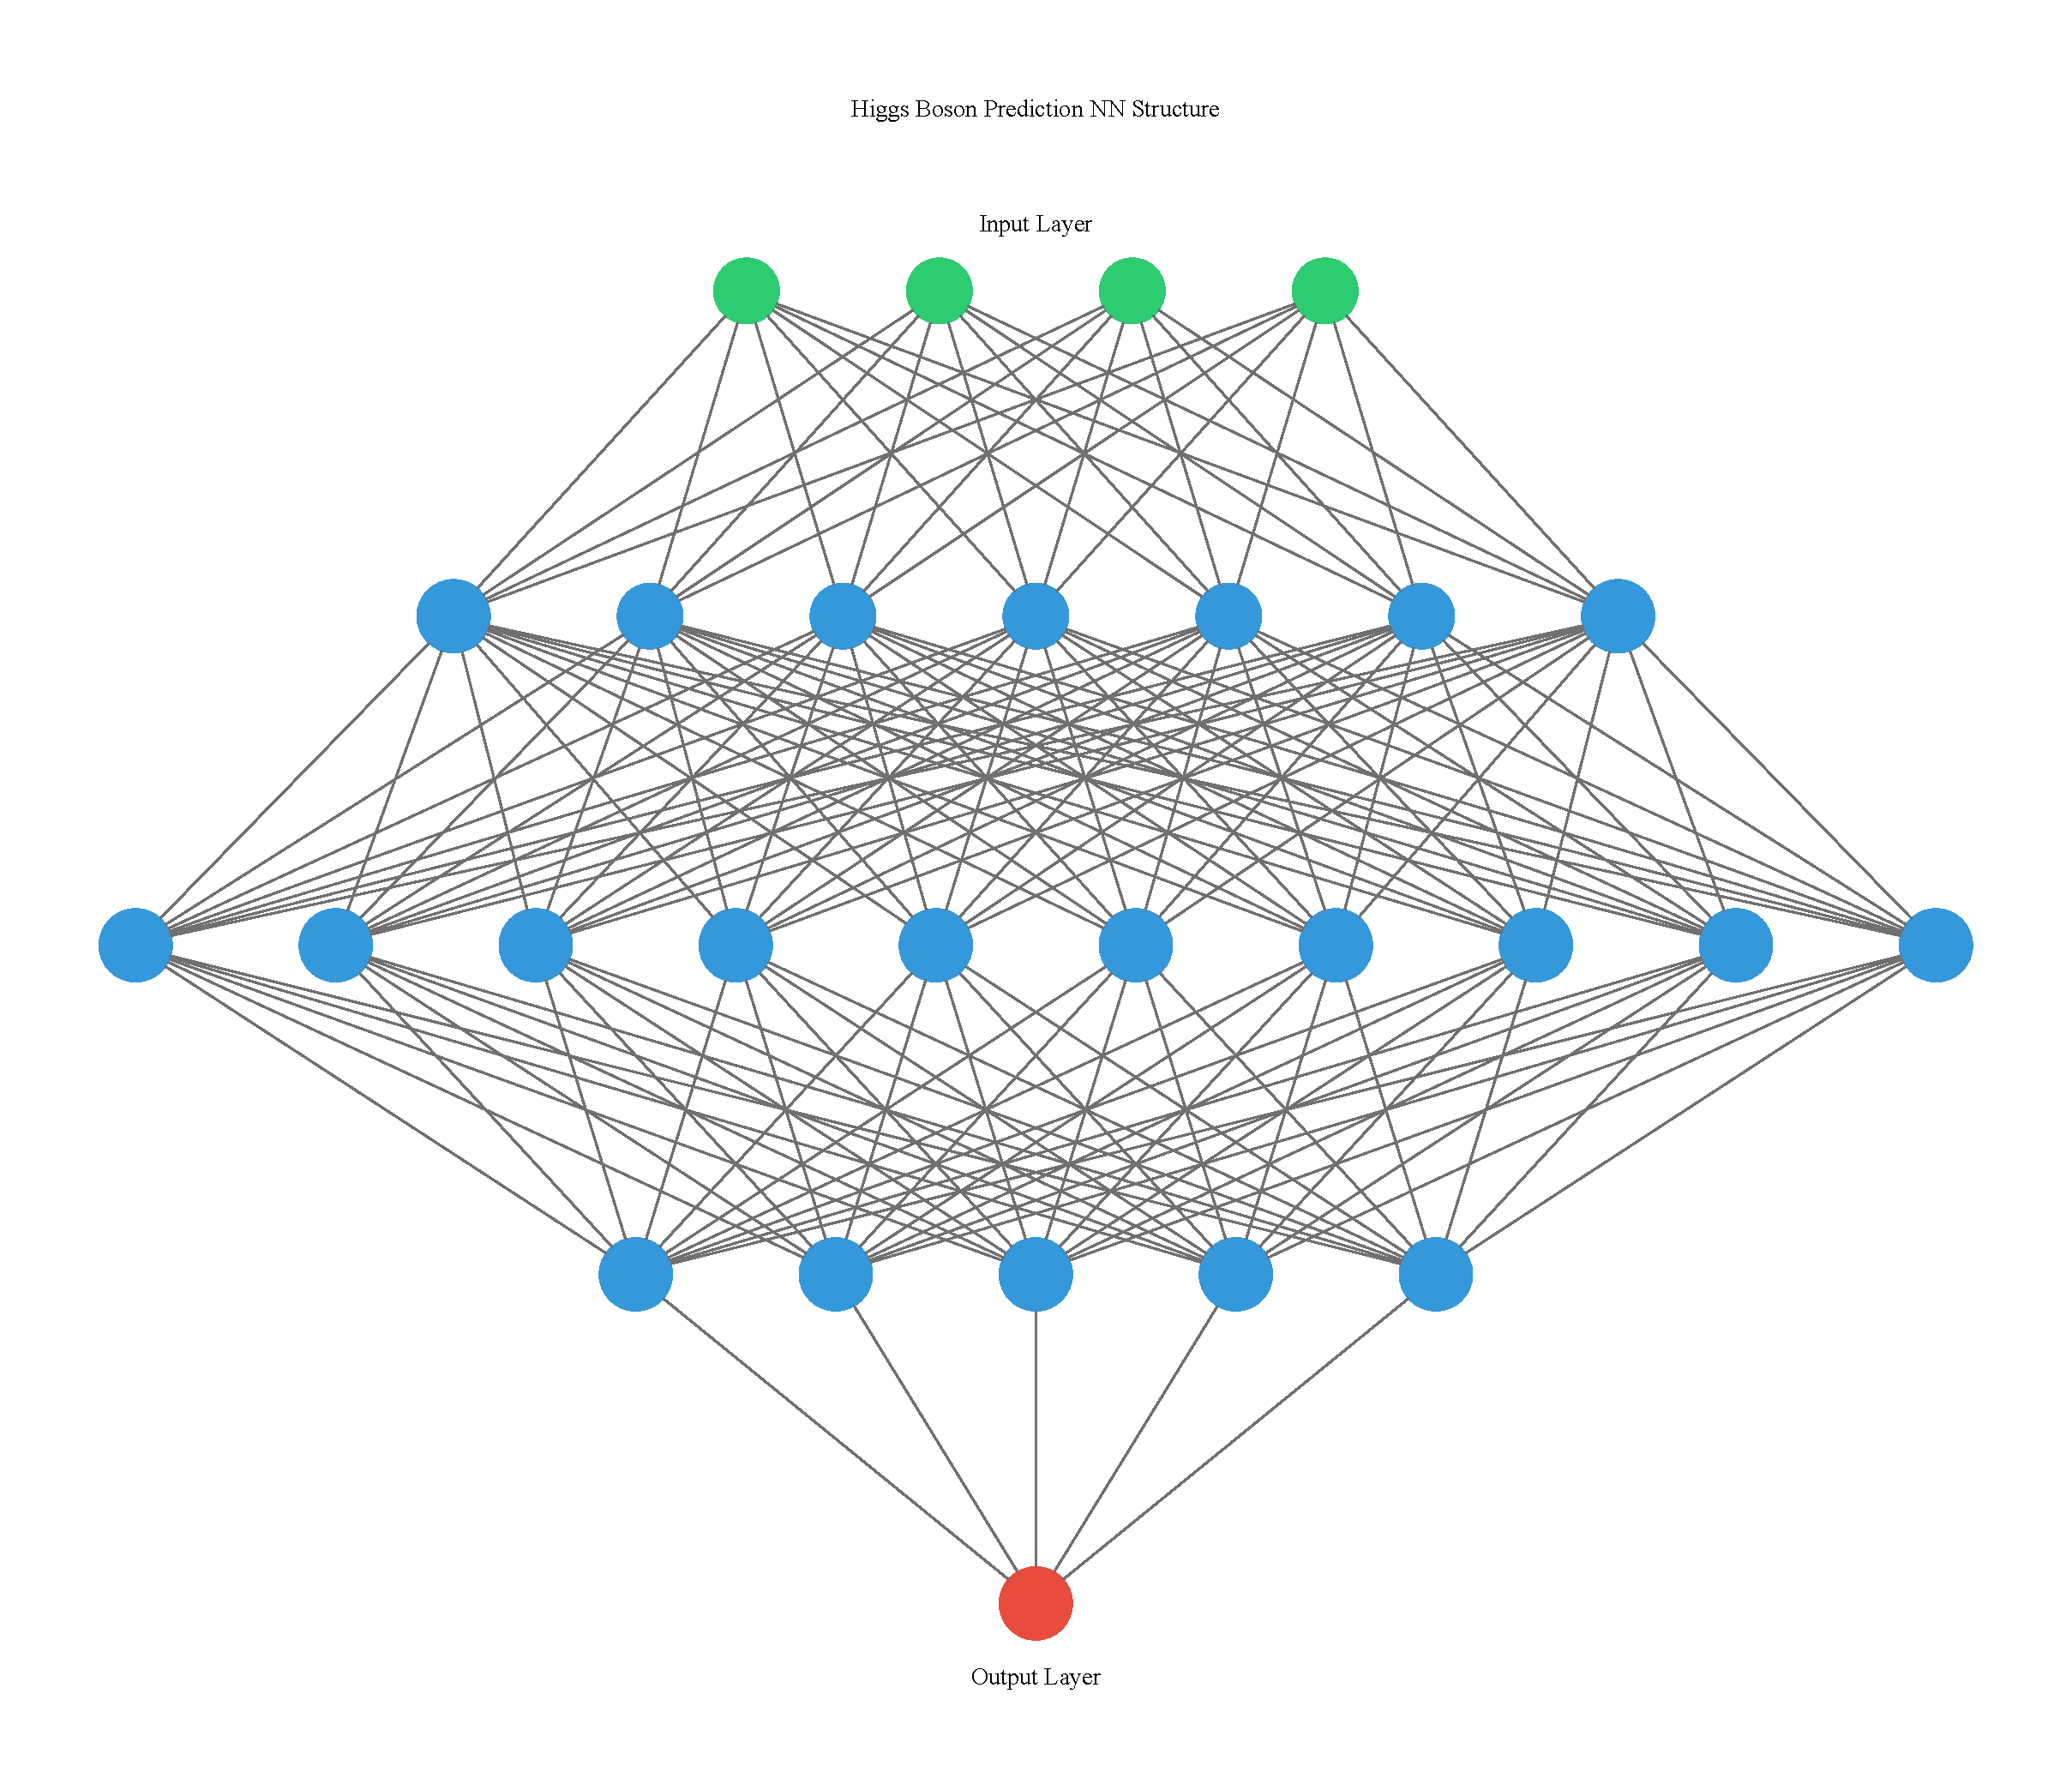
\includegraphics[width = 4in]{My_NN_Structure.pdf}
\caption{Higgs Boson Prediction NN Structure}\label{My_NN_Model}
\end{figure}

In my Neural Network, I use three all-connected hidden layers. And the input features is the total number of particle in one event, the total invariant mass of one event, the number of photon in one event, and the number of ``Muon'' and ``Anti-muon'' in one event. The structure is basically a product of try and error method. The reason I use the ``number of Photon'' and ``number of Muons'' is because although the Higgs boson may decay into these particles, the chances is very small ($0.2\%$ and $0.022\%$).
%
\newpage
%
\section{Result}
\begin{figure}[H]
\centering
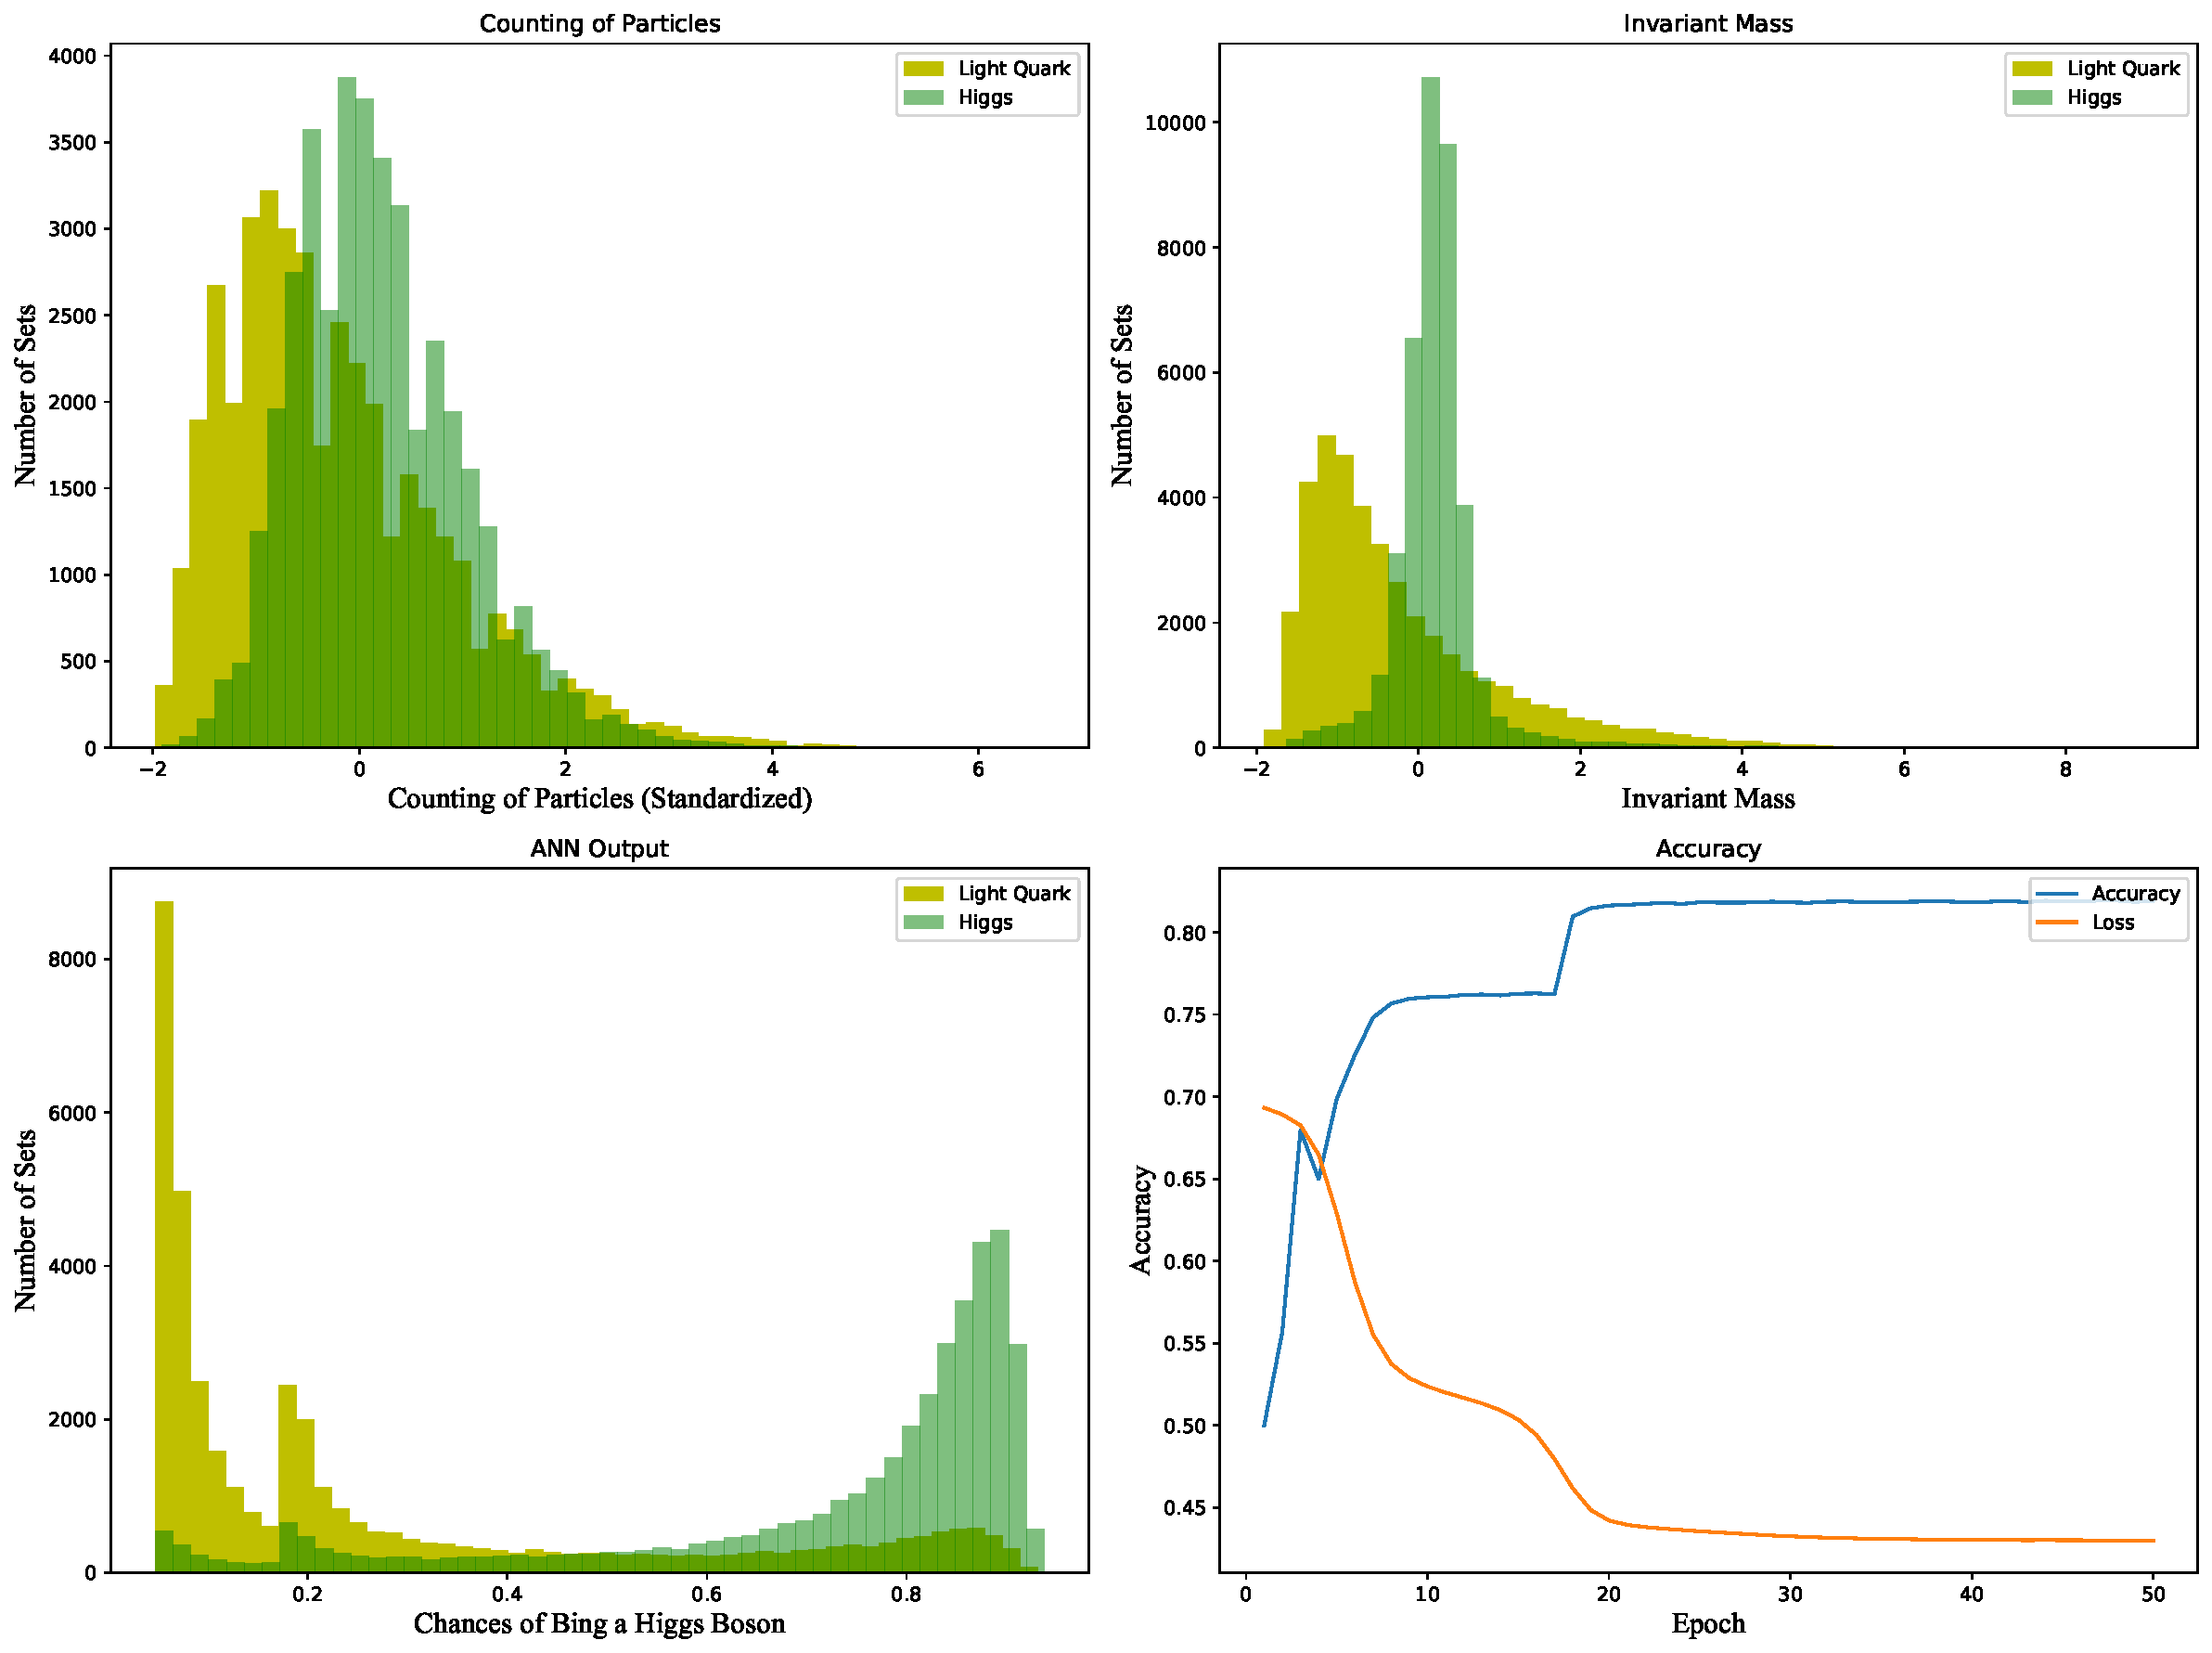
\includegraphics[width = 6in]{Result.pdf}
\caption{NN Model Prediction Result}\label{LHC_Computer_Simulation}
\end{figure}

As you can see in the Figure \ref{My_NN_Model}, after aboue $30-40$ epoch, the accuracy of my model converged at about $81\%$.
%
\newpage
\section{Conclusion}
This project is primarily aimed at predicting Higgs boson using deep learning methods. The Higgs boson, a fundamental particle confirmed in 2012, plays a vital role in the formation of the standard model and the deepening understanding of physics. Our objective is to explore how deep learning can be more effectively applied in the field of particle physics, specifically for the prediction of Higgs boson.

Currently, our deep learning model has achieved an accuracy rate of approximately 81\%. This result is commensurate with the current average level in the field, indicating that our model has acquired basic predictive capability. However, considering the challenges of Higgs boson prediction and the potential of deep learning, I believe there are still possibilities for further enhancement of the model performance.

In future work, I will focus on further optimization and enhancement of the model. This will involve adjusting the parameters of the deep learning model, adding more features related to Higgs boson, and optimizing the model's training strategy. I believe that through these improvements, T will be able to increase the model's predictive accuracy.

In addition, I will conduct a more in-depth analysis to understand the situations in which the model's predictive capability is weaker, to identify areas needing improvement. This will help us more accurately locate the problem and optimize it in a targeted manner.

I also hope to further deepen the application of deep learning in the field of physics and attempt to apply this technology to more physical problems. I believe that this will not only help promote the development of physics, but will also broaden the application scope of deep learning.

In conclusion, although our model has only barely reached the average level at present, I are still confident about the future possibilities. I will continue to optimize our model and apply deep learning technology.

\newpage
\bibliographystyle{unsrt}
\bibliography{bibliography.bib}

\end{document}



















